\chapter{Project Description}

\label{ch:problem}

Over the centuries, knowledge has been fundamental to any learning process. Socrates already stated that knowledge is the only true virtue, and the tragedian Aeschylus regarded memory as the mother of all knowledge. Moreover, it was not only regarded as important by ancient thinkers, but is still regarded as such by modern scholars on education. The taxonomy of learning by \citeA{bloom}, a revision of the taxonomy by \citeA{krathwohl}, and the three stages of skill acquisition by \citeA{skillacquisition}, propose that all learning should start with memorising factual knowledge. Furthermore, \citeA{glaserfield}, one of the main founders for critical constructivism, expresses a need for training students so that they permanently possess facts and are able to repeat them flawlessly whenever they are needed, while also understanding what is placed into their memory. \citeA{ltwm} adds to this by stating that in order to perform complex tasks, people must maintain access to large amounts of information, and that solely encoding knowledge is not sufficient. Despite all of this, \citeA{karpicke4} argues that ``[r]etrieval processes, the processes involved in using available cues to actively reconstruct knowledge, have received less attention'' (p. 158), whereas basic research on learning and memory has emphasised that retrieval must be considered in any analysis of learning.

Traditionally, when students have to gain complex and meaningful knowledge -- for example knowledge about a historical event or a chapter in a psychology textbook, they are asked to read the relevant chapter from a provided textbook. However, \citeA{learninginstruction} states that many students have difficulty gaining knowledge in this manner. He breaks reading for comprehension down into four separate skills, which are integrating, organising, elaborating, and monitoring. Integrating refers to relating a text to one's prior knowledge, for which evidence exists that rich background knowledge leads to better inferences about the text, and thereby to better comprehension. This need also has been stressed by \citeA{ausubel}, and forms different problems between individual readers having access to different background knowledge. After integration, the reader has to organise the text, so that the important ideas and the relationships among them are identified. This is mainly a problem for less experienced readers, possessing fewer strategies to quickly identify important parts and thereby spending too much time on reading unimportant information. While organising a text, the student also has to make necessary inferences while reading, or has to elaborate, which is quite difficult for readers when not prompted to do so. Finally, students have to monitor their comprehension, which refers to evaluating their understanding of the text and if necessary adjusting the reading strategy. This is again quite difficult for the average reader, however this can be trained.

While intergrating is something more dependent on the curriculum design, organising and elaborating can be facilitated by a technique called concept mapping, and monitoring by so-called flashcard systems. Furthermore, the flashcard system might be helpful for the integration of a next topic with the current. This research aims to develop a new tool combining these learning tools. In this chapter, concept mapping and flashcard systems be explored on a practical level in order to establish their definitions together with a summary of arguments in favour or opposition of using them as tools for studying textual material, while also describing their current applications within education. Furthermore, a new tool called the flashmap system is introduced.

\section{Concept mapping}
\label{sec:intro_cmap}

A Concept map is a learning tool deviced by Joseph Novak in 1970's, based on constructivist theories of learning. It was originally intended for assessing the structure of student conceptions, before and after instruction, in order to map their prior knowledge and compare it to what they learned during the instruction. This expanded on the notions of \citeA{ausubel}, who stated that what the learner already knows is most important, and that this had to be ascertained before teaching. Although the use of concept maps as an assessment tool remains prevalent \cite{canas, chung, hwang2, ruiz1}, over time, students began to use it as a tool to comprehend textual material by organising and elaborating on the included concepts \cite{canas, eppler, hwang2, karpicke2, nesbit}.

\subsection{Definition}

One definition provided by \citeA{burdo} states that "concept maps are hierarchical representations of knowledge. Construction of them involves linking concepts [...] through the use of linking phrases into propositional statements" (p. 335). The concepts are typically nouns or verbs with or without modifying adjectives or adverbs, and linking phrases specify the relationship between two concepts. \citeA{ruiz1} also mention these elements in their own definition, yet \citeA{canas} and \citeA{eppler} include a few extra features, such as the concepts being ordered in hierarchical fashion. They describe two different kinds of links, which are hierarchical links to indicate ranking between the concepts, and crosslinks to indicate relationships between concepts in different segments or domains of the concept map. The latter aims at relating concepts residing within different knowledge domains, enabling better connections to prior knowledge of the learner. According to \citeA{eppler}, concept maps are always top-down and show systematic relationships among sub-concepts relating to one main concept, however \citeA{canas} state that they can also be cyclical as long as the concepts still have a conceptual hierarchy. Finally, most of the above mentioned articles describe the links between concepts to be directed. In conclusion, the definition of concept maps used within this thesis will be:

\begin{definition}
    A concept map refers to a directed graph, in which the nodes consist of concepts, and the edges of -- either hierarchical or cross- -- links labeled with linking phrases, forming several propositional statements about a knowledge domain.
\end{definition}

\noindent An example of a concept map is displayed in figure~\ref{fig:conceptmap}.

For this study, the more interesting aspects of concept maps are the use of concept mapping for elaborating, and of demonstrating meaningful relationships between concepts to learners. The first use of the concept map is known as generative use, and the second as supplantive \cite{instructionaldesign}.

\begin{figure}
    \centering
    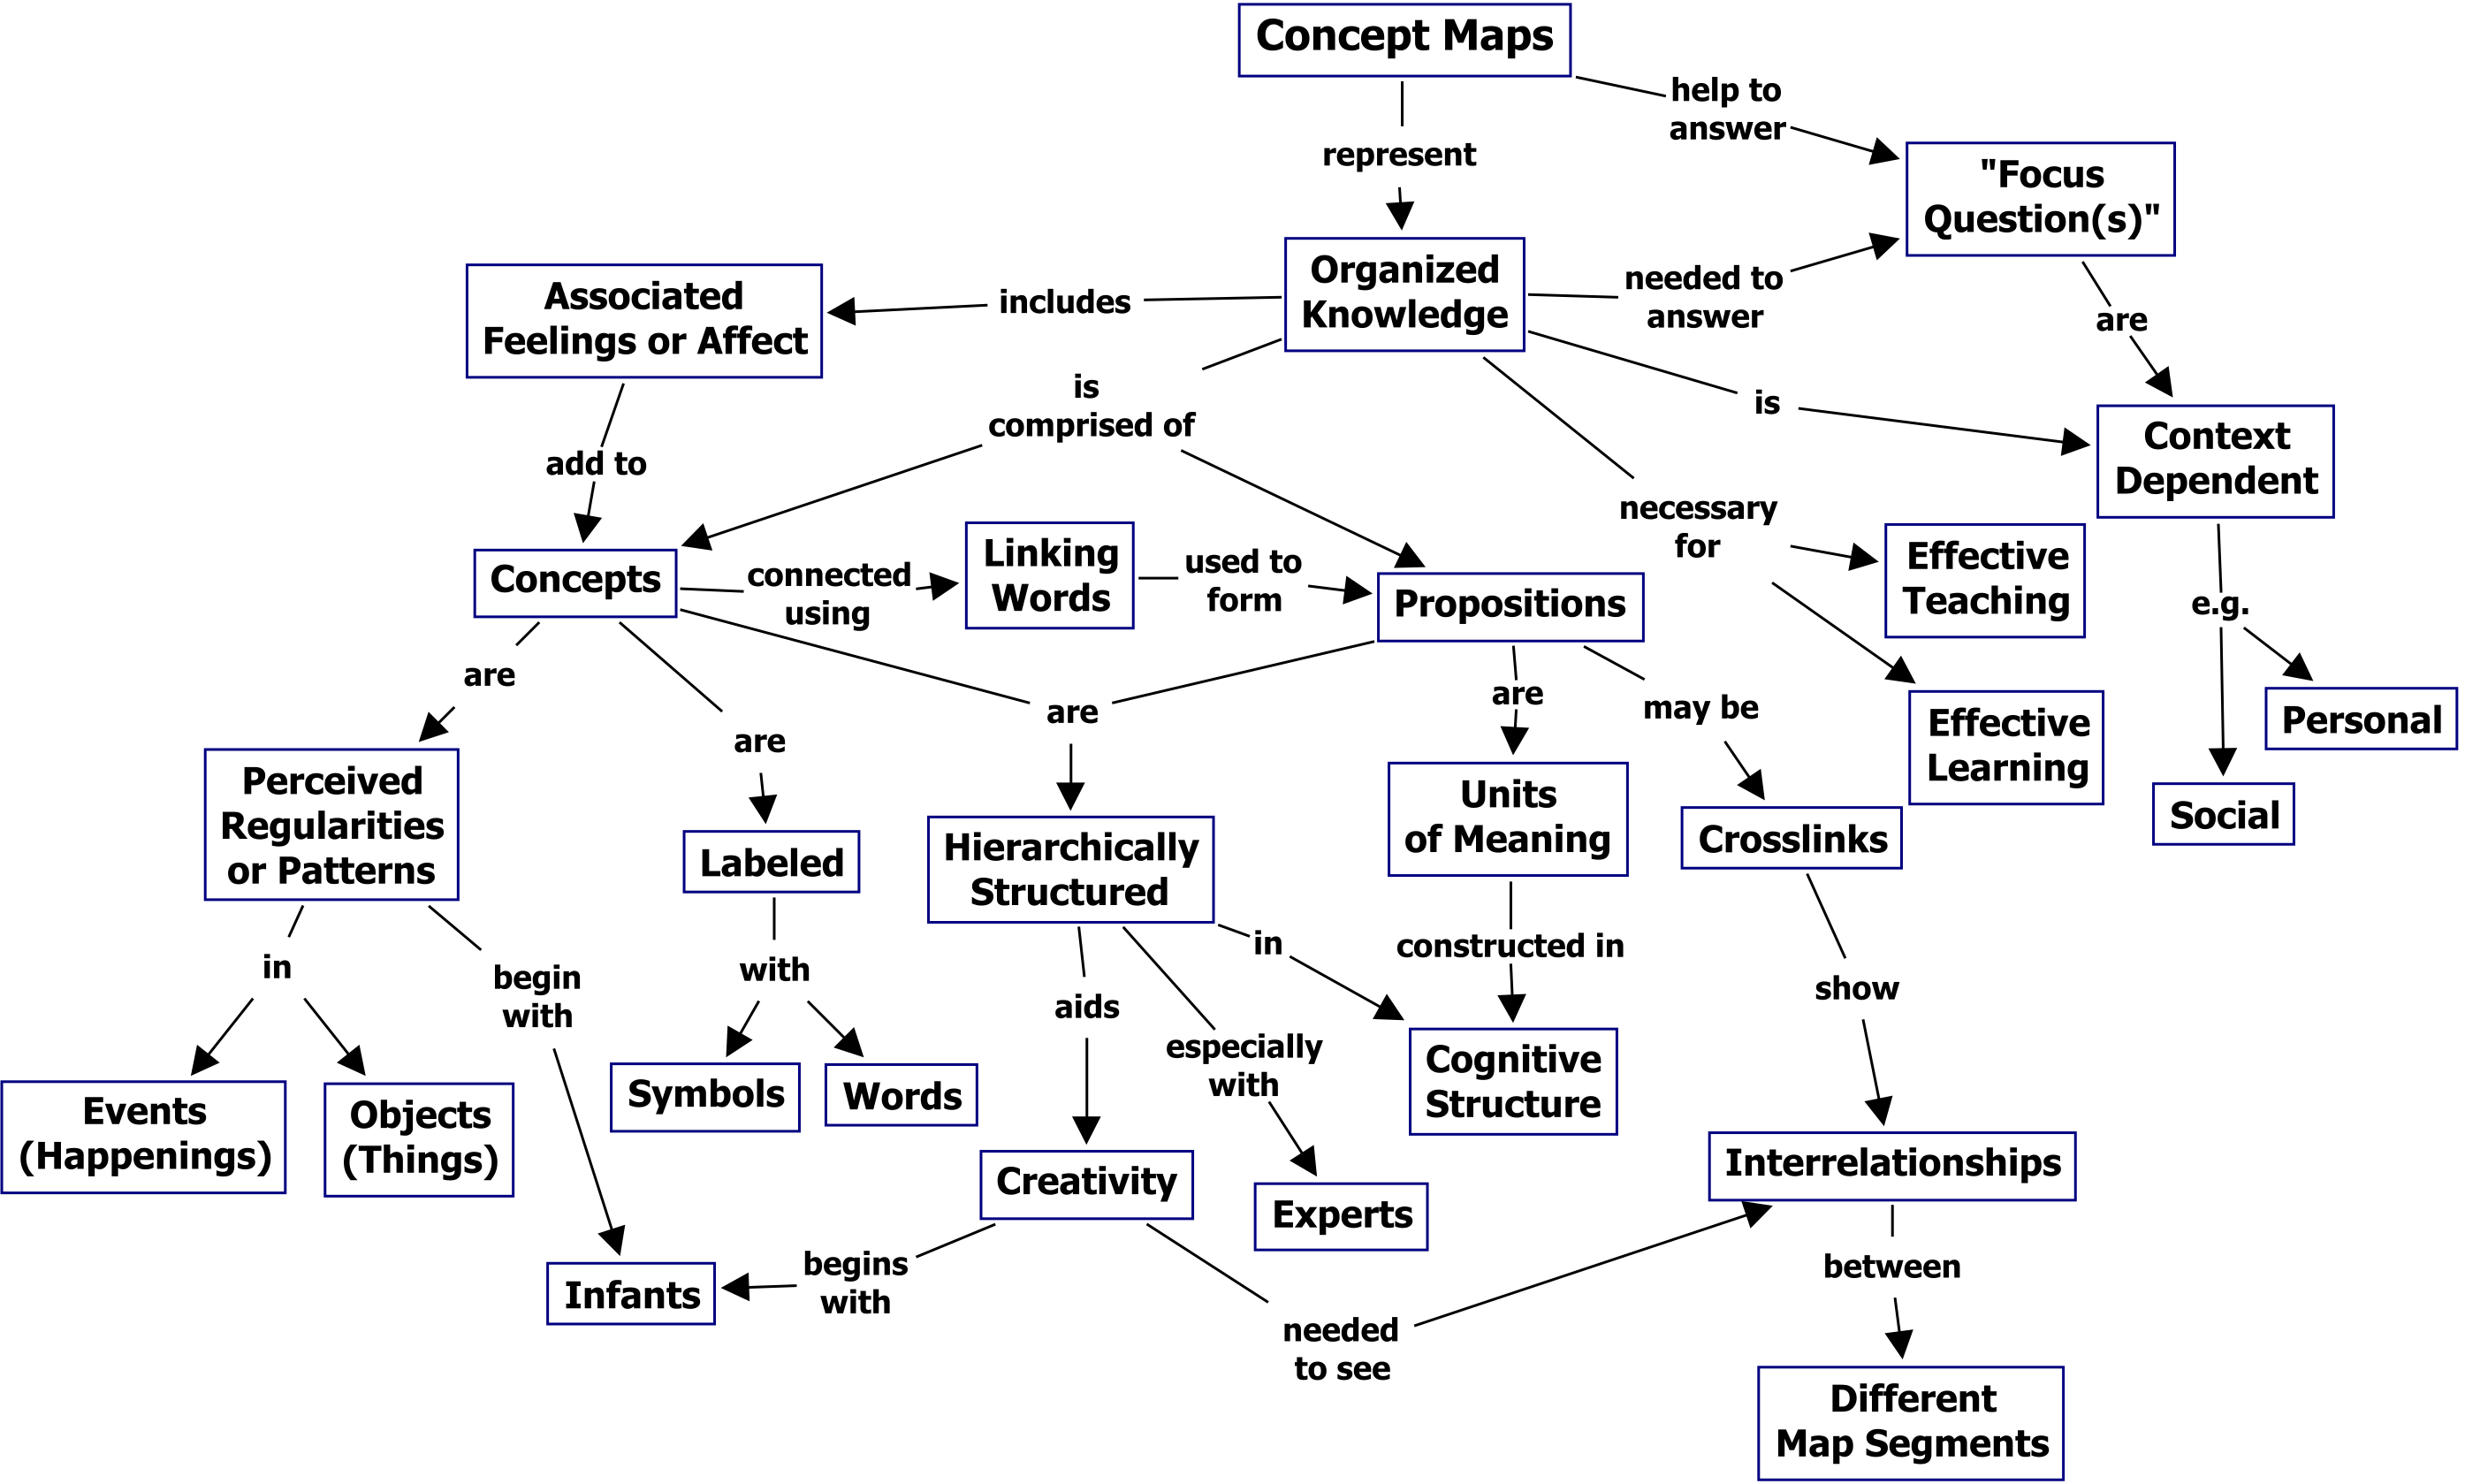
\includegraphics[width=\textwidth]{img/conceptmap.png}
    \caption{An example of a concept map by \protect\citeA{constructcmaps}}
    \label{fig:conceptmap}
\end{figure}

\subsection{Effectiveness}

Multiple studies, both qualitative and quantitative, have demonstrated that concept maps can promote meaningful learning \cite{canas, hwang2, nesbit, subramaniam, singh}. One of the positives of the concept map is that it does not provide learning by means of disconnected facts, but rather as a cohesive narrative placing emphasis on the connections between the concepts. However, most studies state that merely studying a concept map (supplantive use) is not sufficient, and that constructing the concept map (generative use) is essential for using it as a learning tool. However, no studies were found testing this hypothesis, and yet \citeA{blankenship} have found that expert generated concept maps do help students gain conceptual understanding. Still, this study did also indicate that greater maps (more than 20 nodes) used within textbooks lead to \emph{map-shock}, which \citeA{moore} defines as ``a type of cognitive overload that prevents students from effectively processing the concept map, thereby inhibiting their ability to learn from it'' (p.~3). Finally, \citeA{eppler} enlists some of the main advantages and disadvantages in comparison to other visualisation formats (mind maps, conceptual diagrams, and visual metaphors). A positive aspect is that students can gain information rapidly, because of the systematic, proven approach to provide an overview and the emphasis on relationships and connections among concepts. On the other hand, the technique of concept mapping is not easy to apply by novices and requires exstensive training, since otherwise the maps tend to turn out to be idiosyncratic. Furthermore, although better understandability is provided, the overall pattern does not necessarily assist memorability. Finally, the quality of concept maps can be assessed through evaluation rules, however this turns out to be quite a time consuming task for the tutors.

\section{Flashcard system}
\label{sec:intro_fc}

In contrast to concept maps, a flashcard system is not intended for meaningful knowledge encoding, but rather for the rehearsal of knowledge so that it keeps active and as such is prevented from being forgotten.

\subsection{Definition}

In the context of language learning, \citeA{nakata} defines flashcard systems as learning tools in which ``target items are presented outside meaning-focused tasks, and learners are asked to associate the L2 [foreign language] word form with its meaning, usually in the form of a first language translation, L2 synonym, or L2 definition'' (p. 17). This form of learning is also referred to as a \emph{paired-associate format}, which refers to learning by the learner being presented by cues and having to recall an associated counterpart. Besides vocabulary learning, it can also be used to memorise word definitions or topographical information. In order to be more inclusive of other use cases, the following general definition is proposed:

\begin{definition}
    A flashcard system refers to any system in which a learner is presented with cues and has to recall their counterparts from a paired-associate format.
\end{definition}

The most simple form of a flashcard system is a system where the learner has a stack of cards, with each containing a retrieval cue on one side and the correct associated response on the other side. A learning session then consists of going through the whole stack each day and trying to come up with correct answers. Efficiency can then be increased by repeating difficult cards more often, or skipping reviewing certain easy cards for multiple days. This way, the learner only focuses on the pairs which require more practice. Finally, the size of the stack of cards can be increased over multiple days in order to improve the spreading of cognitive load. Next to these paper flashcards, there is also a multitude of digital flashcard systems available \cite{hwang2, nakata, microlearning}, which allow for automating the rescheduling of flashcards and thereby providing better access to more advanced algorithms.

\subsection{Effectiveness}

Flashcard systems have not been completely free from criticism by other researchers. \citeA{hulstijn} for example describes flashcards as a relic of the old-fashioned behaviourist learning model, and \citeA{mccullough} states that the main emphasis of flashcards is memorisation, not comprehension. However, \citeA{zirkle} state that it is still important for teachers and students to understand and utilise memory in such a way that a store of knowledge is produced that remains flexibly retrievable in a variety of contexts over a period of time. Flashcards have been found to be both a time efficient tool for learning large numbers of facts and an effective tool for these facts to be more resistant to decay in comparison to traditional teaching methods \cite{nakata}. Furthermore, \citeA{kornell} state that ``perhaps no memorisation technique is more widely used than flashcards'' (p.~125). Their effectiveness also has been demonstrated accross studies in different contexts, for example that of language learning \cite{chien, macquarrie, mccullough, nakata}, word recognition \cite{joseph}, psychology courses \cite{burgess, golding}, and geography \cite{zirkle}. Therefore, many authors support pursuing research into flashcards and its effective application into classrooms.

\section{Comparison of the two tools}
\label{sec:comparison}

In summary, most studies describe concept mapping as a tool for meaningful encoding, whereas flashcards are described as a tool for rote memorisation, and therefore imply that the former approach leads to more comprehension than the latter. A recent study by \citeA{karpicke2} researched this hypothesis by having participants study a science text with four different learning conditions and prompting them afterwards with verbatim and inference questions and metacognitive predictions. Within the first condition, students only had to read the text and then answer the quesions. The second group studied the text repeatedly in four consecutive study periods. Students within the third group studied the text in one initial study period and then created a concept map after being instructed in concept mapping. The final group studied the text in an initial study period and then had to retrieve as much from the text as they could on a free recall test. The time spent on concept mapping and recalling was equal. When analysing the results, it was found that the retrieval group performed highest on both the verbatim and the inference questions, whereas the repeated study and concept mapping groups performed about equally well and the study once group performed the worst. Interestingly enough, the retrieval group judged their own learning the lowest, and the repeated study group the highest. The same effect of concept mapping and retrieval practice was found again in a second reproduction study, and also in another study by \citeA{burdo}. It is theorised that during elaboration, subjects attain detailed representations of encoded knowledge by linking concepts together in meaningful ways, but that during retrieval, subjects use retrieval cues to reconstruct meaning en thereby already organise the content in a meaningful way. \citeA{karpicke2} conclude that these insights could pave the way for the design of new educational activities with retrieval practices in mind.

\section{Flashmap system}
\label{sec:intro_flashmap}

It can be concluded that both of these tools are helpful for studying, since concept maps help students organise by drawing hierarchical links and elaborate on the content by drawing cross-links, and flashcards help students monitor their understanding of the text and retain the knowledge in order to facilitate integration with a following topic where the knowledge may prove relevant. The object of this study is therefore to create a new digital learning tool, referred to as Flashmap system, that combines both the visual overview of concept maps with the retrieval mechanism of flashcard systems. It will present incomplete parts of a concept map, in which the student has to fill in the missing parts of propositions represented by that map (see figure~\ref{fig:flashmap}). These parts will consecutively be repeated according to algorithms already used by digital flashcard systems. Thereby, the system should make the relations between the concepts explicit to the student, increasing the organisation of the knowledge and reducing the segregation of facts. Because of this, the system might have the potential to bridge the gap between the two systems, and therefore make meaningful and effective rote memorisation possible, facilitating the needs stressed by both \citeA{karpicke4} and \citeA{zirkle} of more meaningful retrieval. Furthermore, by having the students memorise the concept map and graduately expanding on it, the generally experienced map shock occuring with expert-generated concept maps might also be mitigated (see also \citeNP{tzeng}).

\begin{figure}
    \centering
    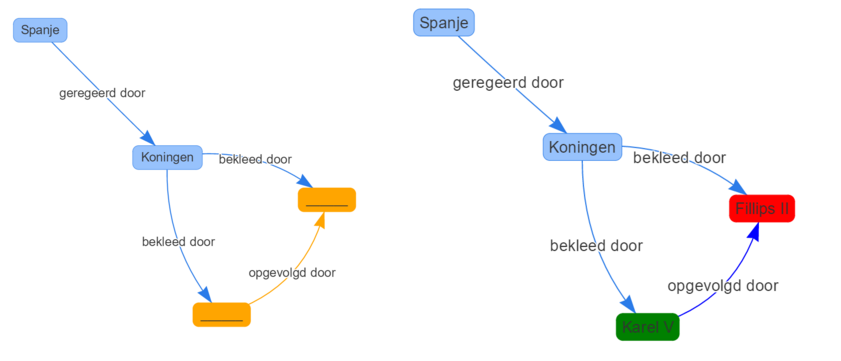
\includegraphics[width=\textwidth]{img/flashmap}
    \caption{A display of the flashmap system, where the user has to think of the concepts fitting in the orange nodes on the left, and has to indicate which nodes were correct on the right}
    \label{fig:flashmap}
\end{figure}

\section{Evaluation}

\label{sec:intro_evaluation}

This project does not only aim to develop a flashmap system, but also to evaluate it by comparing it to a similarly functioning flashcard system. Since the retrieval practices have already been established to be more effective than concept maps (see the \nameref{sec:comparison} section), the flashmap system is only evaluated in comparison to a similarly functioning flashcard system. The group approached for participating within the evaluation constists of Dutch high school teachers of the Stedelijk Lyceum has been found willing to participate, with their students using either the flashmap or the flashcard system for self study parallel with classroom instruction. The content of the instruction is Dutch literature during the sixteenth and seventeenth century, to be learned by the students for a school exam. For example, the students have to learn what the influence was of the Dutch War of Independence on the \emph{Spaanschen Brabander} by Bredero. Because of the content existing mainly of concepts with meaningful relations it fits to the concept map technique, and thereby the flashmap system could be significantly beneficial over the flashcard system.

\newcounter{researchquestion}
\renewcommand{\theresearchquestion}{\Roman{researchquestion}}
\newcounter{subquestion}[researchquestion]
\renewcommand{\thesubquestion}{\alph{subquestion}}

The research aims to investigate the following questions: Regarding high school students learning for Dutch literature using the flashmap system in comparison to them using the flashcard system\ldots
%
\refstepcounter{researchquestion}\label{benefit}
\refstepcounter{subquestion}\label{effectiveness}
\Roman{researchquestion}\alph{subquestion}. \ldots is the learning gain larger?
%
\refstepcounter{subquestion}\label{efficiency}
\Roman{researchquestion}\alph{subquestion}. \ldots have they spent about equal time on the software?
%
\refstepcounter{researchquestion}\label{perception}
\refstepcounter{subquestion}\label{usefulness}
\Roman{researchquestion}\alph{subquestion}. \ldots do they perceive the system to be more useful?
%
\refstepcounter{subquestion}\label{ease}
\Roman{researchquestion}\alph{subquestion}. \ldots do they perceive the system to be easier to use?
%
Whether the flashmap system is more effective than the flashcard system is measured by the learning gain of high school the students, referring to the knowledge obtained by a student over the course of an instruction. Sequentially, the efficiency of the system is determined by the material covered by the users, and the amount of time spent on the system.

For measuring the affectiveness of the systems, the Technology Acceptance Model by \citeA{tam} will be used (see figure~\ref{fig:tam}). This model predicts the use of an information system by measuring the Perceived Usefulness and the Perceived Ease of Use of the user. These variables are mediators between External Variables and Attitude towards using, leading to Behavioural intention to use, which in turn leads to the Actual system use.

\begin{figure}
    \centering
    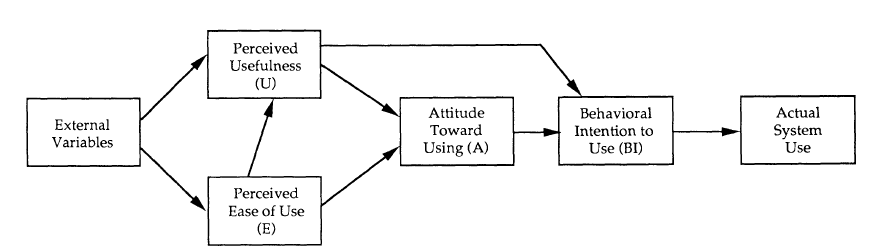
\includegraphics[width=\textwidth]{img/tam}
    \caption{The Technology Acceptance Model by \protect\citeA{tam}}
    \label{fig:tam}
\end{figure}

Answering the research questions has both practical and scientific relevance. From a practical perspective, it has potential to overcome the criticism from various authors about flashcard systems and answer the need for meaningful rote memorisation. From a scientific perspective, it can provide new insights on the way students learn texts. Finally, it makes way for new research opportunities, for example what the difference in effect is of when the user develops their own concept maps or flashcards to be used within the system, or when they are created by the teacher or an expert. 

The following chapter will elaborate further on the cognitive theories underlying concept mapping and flaschard systems on page~\pageref{ch:theory}, after which the design and development of the flashmap will be described in part II. Finally, the research conducted within this project and its results will be described in part III.
